\documentclass[a4paper,10pt]{article}

\usepackage{graphicx}
\usepackage{amsmath}
\usepackage[latin1]{inputenc}
\usepackage[spanish]{babel}

\title{ \textbf{ 6620. Organizaci\'on de Computadoras\\
Trabajo Pr\'actico 1: \\
Conjunto de instrucciones MIPS}}

\author{	Gonz\'alez, Juan Manuel, \textit{Padr\'on Nro. 79.979} \\
            	\texttt{ juan0511@yahoo.com } \\[2.5ex]
            	Arg\"uello, Osiris, \textit{Padr\'on Nro. 83.062} \\
            	\texttt{ osirisarguello@yahoo.com.ar } \\[2.5ex]
		Paez, Ezequiel Alejandro, \textit{Padr\'on Nro. 84.474} \\
		\texttt{ skiel85@gmail.com } \\[2.5ex]
            	\normalsize{1er. Cuatrimestre de 2012} \\
            	\normalsize{66.20 Organizaci\'on de Computadoras  $-$ Pr\'atica Jueves} \\
            	\normalsize{Facultad de Ingenier\'ia, Universidad de Buenos Aires} \\
       }

\date{}

\begin{document}
\maketitle
\thispagestyle{empty}  % quita el numero en la primer pagina

\begin{abstract}
El presente trabajo pr\'actico tiene como objetivo familiarizarse con el conjunto de instrucciones MIPS32 y el concepto de ABI, desarrollando para ello un programa que implemente el algoritmo de ordenamiento \textit{mergesort}.
\end{abstract}

\pagebreak

\setcounter{page}{2}
\section{Introducci\'on}
El presente trabajo tiene como objetivo familiarizarse con el conjunto de instrucciones MIPS32 y el concepto de ABI. Se utilizar\'a el programa GXemul para simular un entorno de desarrollo en una m\'aquina MIPS (corriendo una versi\'on del sistema operativo NetBSD).\\
Se desarrollar\'a, en lenguaje assembly, un programa que implemente el algorimto de ordenamiento \textit{mergesort}. La implementaci\'on de este trabajo pr\'actico debe tomar entrada exclusivamente desde \textit{stdin}. La salida debe imprimirse por \textit{stdout}, mientras que los errores deben imprimirse por \textit{stderr}.\\

\section{Programa a implementar}
Al igual que el TP0, el presente trabajo pr\'actico tiene como objetivo implementar el algoritmo de ordenamiento \textit{mergesort}, esta vez en assembly de MIPS32. La implementaci\'on de este trabajo pr\'actico debe tomar entrada exclusivamente desde \textit{stdin}. La salida debe imprimirse por \textit{stdout}, mientras que los errores deben imprimirse por \textit{stderr}.\\
Asimismo, la implementaci\'on a realizar debe respetar la ABI usada por la c\'atedra[7], que difiere de la utilizada por el GCC.\\
Por otro lado, para hacer uso de memoria din\'amica, se ha provisto junto con el enunciado de una implementaci\'on de \textit{malloc} y \textit{free} escrita en assembly MIPS32. La funci\'on \textit{realloc} debe ser implementada como parte del trabajo pr\'actico.\\
Finalmente, para poder realizar el trabajo pr\'actico, ser\'a necesario interactuar con el sistema operativo mediante las llamadas al sistema SYS\_read y SYS\_write por medio de \textit{syscalls}. Los pasos necesarios para lograr esto fueron expuestos en clase durante la explicaci\'on del enunciado del trabajo:

\begin{itemize}
\item 
Cargar el n\'umero de llamada al sistema en el registro \$v0.
\item
Cargar los argumentos en los registros correspondientes. 
\item
Ejecutar la llamada mediante la instrucci\'on \textit{syscall}.
\item
Verificar la existencia de errores en el registro \$a3.
\item
Obtener el valor retornado del registro \$v0.
\end{itemize}

La c\'atedra ha adjuntado al enunciado del trabajo pr\'actico una versi\'on minimalista del comando echo de UNIX a modo de ejemplo.

\pagebreak

\section{Consideraciones sobre el desarrollo}
A continuaci\'on se detallan las consideraciones tenidas en cuenta para el desarrollo del trabajo pr\'actico. Hemos decidido separar las que surgen del Dise\~no de las que surgen en la Implementaci\'on.

\subsection{Consideraciones de Dise\~no}
El programa desarrollado para resolver el presente trabajo pr\'actico consta a grandes rasgos de un int\'erprete de l\'inea de comandos (simplemente verifica que no se pasen argumentos al programa), la rutina que lee los datos de entrada desde \textit{stdin}, una estructura de datos dise\~nada para almacenarlos, la funci\'on encargada de efectuar el ordenamiento y finalmente la funci\'on que imprime la salida del programa. Se decidi\'o separar el c\'odigo fuente en una serie de archivos, a modo de mejorar su legibilidad y organizaci\'on. A continuaci\'on se presenta la lista de archivos que componen el proyecto:\\
\\
\begin{tabular}{|l|l|}
\hline
Archivo & Descripci\'on \\ \hline
tp1.S & Funci\'on main e int\'erprete de l\'inea de comandos. \\
manejoes.S & Funci\'on de lectura de entrada y escritura de salida. \\
sort.S & Funci\'on de ordenamiento por \textit{mergesort}. \\
mymemory.S & Funciones adicionales de manejo de memoria din\'amica. \\
mymalloc.S & Implementaci\'on de mymalloc y myfree. \\
io.S & Implementaci\'on de my\_read y my\_write. \\
constantes.h & Definici\'on de las constantes y c\'odigos de error internos del programa. \\
\hline
\end{tabular}\\
\\
\\Dada la similitud del problema a resolver con el TP0, se decidi\'o como punto de partida modificar el c\'odigo de dicho trabajo pr\'actico para hacerlo cumplir con la especificaci\'on del nuevo enunciado. El haber hecho esto permiti\'o contar con una versi\'on del programa implementada en alto nivel para utilizar de gu\'ia a la hora de codificar en assembly MIPS32. Dicha soluci\'on se entrega junto con el presente informe a modo de referencia.\\
La estrategia utilizada, una vez obtenido dicho c\'odigo C, fue la de ir reemplazando cada uno de los archivos fuente por su equivalente codificado en MIPS32, en forma parcial, de manera de ir haciendo pruebas incrementales de la implementaci\'on en assembly. De esta manera, se codific\'o primero el algoritmo de \textit{sort}, y se reemplaz\'o el archivo \textbf{'sort.c'} de la soluci\'on original por uno nuevo, \textbf{'sort.S'}, ya perteneciente a la soluci\'on definitiva. Esto simplific\'o de manera significativa la depuraci\'on del c\'odigo assembly, ya que no eran agregados nuevos archivos codificados en assembly a la soluci\'on final hasta no tener la certeza de que el \'ultimo de los archivos \textbf{.S} agregado funcionara de manera correcta. De esta manera se continu\'o con el desarrollo hasta que fueron reemplazados todos los archivos codificados en alto nivel y el programa cont\'o con la totalidad del c\'odigo desarrollado en assembly.\\
\\En cuanto al dise\~no del programa en s\'i, no difiere en gran parte del TP0, salvo por el hecho de que fueron eliminadas tanto la impresi\'on de la ayuda como la de la versi\'on, y de que en este trabajo los datos de entrada son le\'idos exclusivamente por \textit{stdin}. Para mejorar el \textit{feedback} al usuario, se agreg\'o una validaci\'on sobre el n\'umero argc, de modo que el programa devuelva error si es llamado con alg\'un argumento.\\
Por otro lado, los c\'odigos de error internos al programa fueron actualizados, y tambi\'en se hizo necesario contar con un archivo com\'un no s\'olo para definir dichos valores pero a su vez tambi\'en algunas constantes propias de la operaci\'on del programa, que anteriormente se encontraban en las distintas cabeceras (archivos \textbf{.h}). Dichos valores y c\'odigos fueron definidos en el archivo 'constantes.h'. Su contenido es el siguiente:\\
\\
{\footnotesize \begin{verbatim}
#define stdinfd							0
#define stdoutfd						1
#define stderrfd						2	

#define BUFFER_SIZE						2048

#define ERROR_RESERVA_INICIAL_MEMORIA	2
#define ERROR_RESERVA_MEMORIA			3
\end{verbatim}}

La ejecuci\'on del programa se interrumpe por cualquiera de estos errores, mostrando al usuario un mensaje afin. Los c\'odigos 0 y 1 son utilizados para la devoluci\'on al SO del resultado de la ejecuci\'on, siendo:\\
\\
0: Ejecuci\'on sin problemas.\\
1: Error de ejecuci\'on.\\
\\
Finalmente, cabe destacar que todas las impresiones del programa son ruteadas por \textit{stdout}, y los mensajes de error a trav\'es de \textit{stderr}.\\
\\Si bien se contaba con una implementaci\'on en C, esto no fue suficiente para realizar un pasaje directo a MIPS32, dada la utilizaci\'on en dicho c\'odigo de funciones pertenecientes a la biblioteca est\'andar de C, como por ejemplo \textit{malloc} y \textit{fread} entre otras. En el caso de \textit{malloc} y \textit{free}, la c\'atedra provey\'o un archivo con dichas funciones ya implementadas (\textbf{'mymalloc.S'}), mientras que para la implementaci\'on de la lectura y escritura se aprovech\'o el archivo (\textbf{'io.S'}), tambi\'en entregado junto con el enunciado. Se aclara de todas maneras que para poder utilizar estas dos \'ultimas como parte de la soluci\'on fue necesario corregir parte del c\'odigo, dado que faltaba en ambos casos la instrucci\'on encargada de modificar el \textit{stack pointer} una vez ejecutada la funci\'on.  Distinto fue el caso de las funciones \textit{realloc} y \textit{memcpy}, que debieron ser implementadas como parte del trabajo pr\'actico. Para resolver su codificaci\'on, se repiti\'o el ejercicio descripto anteriormente de logar primero una versi\'on en C y luego realizar el pasaje a assembly.\\
En s\'intesis, el listado de funciones que fueron implementadas en MIPS32 para resolver el TP son:
{\footnotesize \begin{verbatim}
int main(int argc,char **argv)
int mergeSort(char *list,unsigned long length)
void *mymemcpy(void *destination,const void *source,size_t num)
void *myrealloc(void *ptr,size_t old_size,size_t num)
int procesarEntrada(tDynArray *datos_sort)
int imprimirSalida(tDynArray *datos_sort)
\end{verbatim}}

\subsection{Consideraciones de Implementaci\'on}
En esta secci\'on del informe se proceder\'a a exponer los puntos mas relevantes relacionados con la implementaci\'on del trabajo pr\'actico.

\subsubsection{Generaci\'on de ejecutables}
Para generar el ejecutable del programa utilizando la versi\'on implementada en lenguaje C, debe correrse la siguiente sentencia en una terminal:
\begin{verbatim}
$ gcc -Wall -o tp1 tp1.c manejoes.c sort.c
\end{verbatim}

Para utilizar el c\'odigo assembly MIPS32, debe ejecutarse lo siguiente:
\begin{verbatim}
$ gcc -Wall -o tp1 tp1.S manejoes.S sort.S mymemory.S mymalloc.S io.S
\end{verbatim}

N\'otese que para ambos casos se han activado todos los mensajes de 'Warning' (-Wall).

\subsubsection{Descripci\'on del algoritmo de la funci\'on \textit{main}}
La funci\'on main tiene como objetivo la validaci\'on de la sintaxis de ejecuci\'on, la reserva inicial de memoria para la estructura de almacenamiento de los datos de entrada, la llamada a las distintas funciones que tiene el programa y el manejo e impresi\'on de los mensaje de error si se da el caso.\\
\\El planteo de la soluci\'on en MIPS32 comenz\'o mediante el an\'alisis de la implementaci\'on previamente obtenida en C, dando como resultado el stack de la funci\'on y un lineamiento de las estructuras de control a utilizar. Con esto, se procedi\'o a efectuar un proceso de traducci\'on del c\'odigo de alto nivel al assembly, por etapas:

\begin{enumerate}
\item 
Manejo de la creaci\'on y destrucci\'on del \textit{stack} de la funci\'on.
\item
Reserva y liberaci\'on de memoria para la estructura de almacenamiento utilizada.
\item
Llamada a la funci\'on de lectura de datos de entrada.
\item
Llamada a la funci\'on de escritura de la salida del programa.
\item
Llamada al algoritmo de ordenamiento.
\item
Uso del registro \textit{v0}, para detectar el c\'odigo de error devuelto por las distintas operaciones.
\item
Presentaci\'on de mensajes de error al usuario.
\end{enumerate}

Al ser finalizado cada uno de \'estos puntos, se probaba el programa, para asegurar un correcto funcionamiento y evitar los inconvenientes derivados de realizar las primeras pruebas sobre el desarrollo completo.\\
\\Para el resto de las funciones implementadas se sigui\'o una metodolog\'ia an\'aloga, por lo que se presentar\'a solamente el \textit{stack} de cada una de ellas, a menos que sean necesarias aclaraciones adicionales.

\pagebreak

\subsubsection{Diagrama del \textit{stack} de la funci\'on \textit{main}}
A continuaci\'on se muestra el diagrama del \textit{stack} para implementaci\'on en MIPS32 de la funci\'on \textit{main}:

\begin{center}
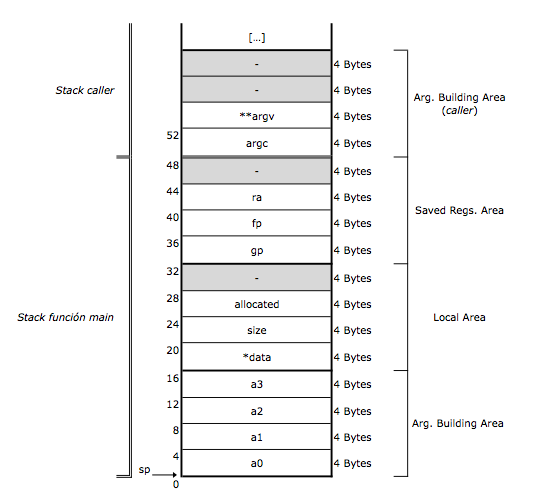
\includegraphics[scale=0.50]{stack_main.png}
\end{center}

\pagebreak

\subsubsection{Diagrama del \textit{stack} de la funci\'on \textit{mergeSort}}
A continuaci\'on se muestra el diagrama del \textit{stack} para implementaci\'on en MIPS32 de la funci\'on \textit{mergeSort}:

\begin{center}
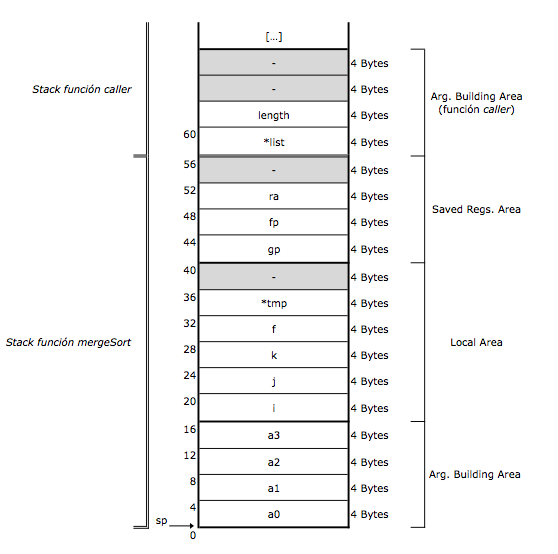
\includegraphics[scale=0.50]{stack_mergeSort.png}
\end{center}

\pagebreak

\subsubsection{Diagrama del \textit{stack} de la funci\'on \textit{procesarEntrada}}
A continuaci\'on se muestra el diagrama del \textit{stack} para implementaci\'on en MIPS32 de la funci\'on \textit{procesarEntrada}:

\begin{center}
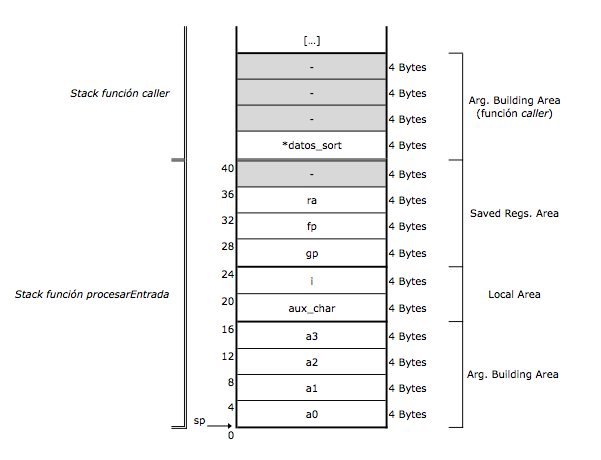
\includegraphics[scale=0.50]{stack_procesarEntrada.png}
\end{center}

\subsubsection{Diagrama del \textit{stack} de la funci\'on \textit{imprimirSalida}}
A continuaci\'on se muestra el diagrama del \textit{stack} para implementaci\'on en MIPS32 de la funci\'on \textit{imprimirSalida}:

\begin{center}
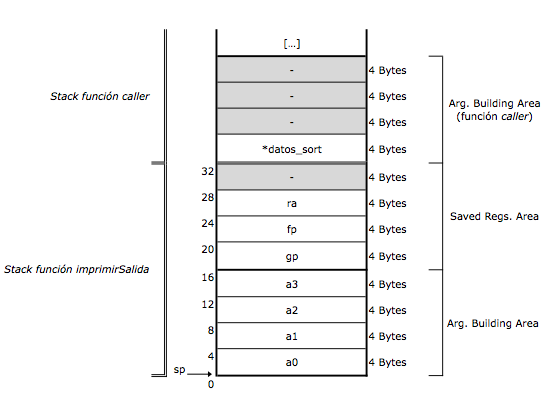
\includegraphics[scale=0.50]{stack_imprimirSalida.png}
\end{center}

\pagebreak

\subsubsection{Descripci\'on del algoritmo de la funci\'on \textit{myrealloc}}
Para la funci\'on \textit{myrealloc} se utiliz\'o como gu\'ia el siguiente c\'odigo, desarrollado en C:

{\footnotesize \begin{verbatim}
void *myrealloc(void *ptr, size_t old_size, size_t size) {

        int minsize;
        void *newptr;
        
        newptr = mymalloc (size);
        if (newptr == NULL)
                return NULL;

        if (ptr != NULL) {
                minsize = old_size;        
                mymemcpy (newptr, ptr, minsize);
                myfree (ptr);
        }

        return newptr;
}
\end{verbatim}}

A diferencia de la implementaci\'on est\'andar, fue necesario agregar un argumento mas, \textit{old\_size}, para conocer el tama\~no del bloque pasado en \textit{*ptr}. Si bien en este trabajo pr\'actico siempre se pide aumentar la memoria reservada, lo que har\'ia innecesario conocer este dato, se prefiri\'o hacer una implementaci\'on con la funcionalidad completa, a costa de no utilizar la definici\'on est\'andar. A su vez, la implementaci\'on elegida requiri\'o la codificaci\'on de \textit{memcpy}, sobre esto se aclara que una optimizaci\'on posible es no ejecutar \textit{memcpy} siempre, ya que si solo se expande el bloque actual la operci\'on es innecesaria.  

\subsubsection{Diagrama del \textit{stack} de la funci\'on \textit{myrealloc}}
A continuaci\'on se muestra el diagrama del \textit{stack} para implementaci\'on en MIPS32 de la funci\'on \textit{myrealloc}:

\begin{center}
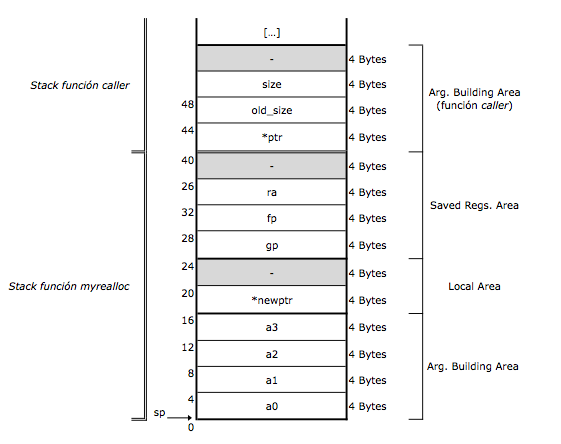
\includegraphics[scale=0.50]{stack_myrealloc.png}
\end{center}

\pagebreak

\subsubsection{Descripci\'on del algoritmo de la funci\'on \textit{mymemcpy}}
La implementaci\'on elegida para \textit{myrealloc} requiri\'o del desarrollo de la funci\'on \textit{memcpy}. A continuaci\'on se presenta el c\'odigo C que fue utilizado como gu\'ia:

{\footnotesize \begin{verbatim}
void * mymemcpy (void * destination, const void * source, size_t num) {

        void * resultado = destination;

        while (num--) {
                *(char *)destination = *(char *)source;
                destination = (char *)destination + 1;
                source = (char *)source + 1;
        }

        return(resultado);
}
\end{verbatim}}

\subsubsection{Diagrama del \textit{stack} de la funci\'on \textit{mymemcpy}}
A continuaci\'on se muestra el diagrama del \textit{stack} para implementaci\'on en MIPS32 de la funci\'on \textit{mymemcpy}:

\begin{center}
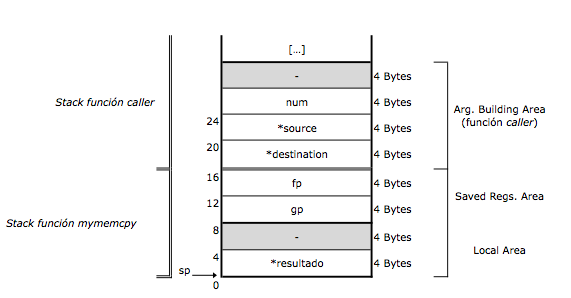
\includegraphics[scale=0.50]{stack_mymemcpy.png}
\end{center}

\pagebreak

\section{Corridas de prueba}
En esta secci\'on se presentan algunas de las distintas corridas que se realizaron para probar el funcionamiento del trabajo pr\'actico.\\
\\
En primer lugar se gener\'o el ejecutable, se comprob\'o el funcionamiento de la validaci\'on de sintaxis de llamada y finalmente se ejecut\'o una prueba trivial:
\begin{center}
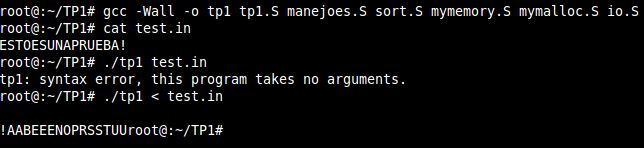
\includegraphics[scale=0.60]{1.png}
\end{center}

Luego, se ejecut\'o la prueba provista por la c\'atedra en el enunciado del trabajo pr\'actico:
\begin{center}
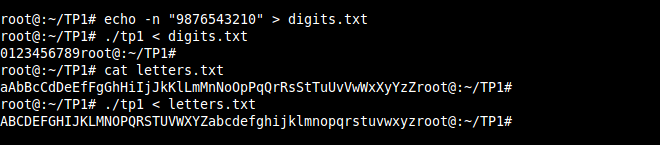
\includegraphics[scale=0.60]{2.png}
\end{center}

\begin{center}
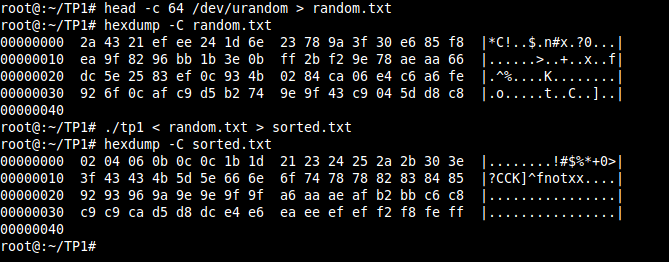
\includegraphics[scale=0.60]{3.png}
\end{center}
\pagebreak

Finalmente, se presenta un ejemplo m\'as mostrando alguna de las salidas posibles, obtenida para casos en los que se trabaja con archivos binarios y cuando se toma entrada por \textit{stdin} en modo interactivo:\\
\begin{center}
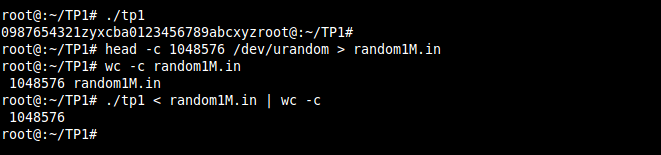
\includegraphics[scale=0.60]{4.png}
\end{center}
\pagebreak

\section{C\'odigo fuente C y MIPS32} 

Tanto el c\'odigo C como el c\'odigo MIPS32 que fue generado en el trabajo pr\'actico ha sido incluido en el CD entregado junto al presente informe.

\pagebreak

\section{Conclusiones}
A modo de conclusi\'on, nos es inmediato resaltar la dificultad que nos ha presentado el programa motivo de este informe. No solo la adaptaci\'on requerida para trabajar con un lenguaje ensamblador y el conjunto de instrucciones del procesador, sino la incorporaci\'on del m\'etodo de programaci\'on que un proyecto de este tipo conlleva.\\

La resoluci\'on del TP nos permiti\'o familiarizarnos a fondo con el conjunto de instrucciones de MIPS32, as\'i como tambi\'en el concepto de ABI. La comprensi\'on de este \'ultimo concepto fue fundamental para el desarrollo de la soluci\'on, ya que en m\'as de una oportunidad nuestro c\'odigo assembly fall\'o por estar mal diagramando el \textit{stack} de la funci\'on a desarrollar. El partir de una implementaci\'on previa como la del TP0 nos impuso la necesidad de investigar formas de resolver la traducci\'on del c\'odigo C utilizando instrucciones que nos eran desconocidas.\\  

Asimismo, consideramos acertada la decisi\'on de haber realizado el desarrollo de la funciones involucradas en la soluci\'on en etapas, con pruebas intermedias como se describe anteriormente, debido a nuestra falta de experiencia con MIPS32. Lo mismo puede afirmarse de haber tomado como gu\'ia el programa desarrollado en lenguaje C.\\

Finalmente, en base a los resultados obtenidos y el tiempo que demand\'o el desarrollo de la tarea, en comparaci\'on con el esfuerzo requerido para resolver el mismo problema en lenguaje C, creemos que no es redituable la demora y dificultad encontrados. Si bien creemos que el TP constituye un ejercicio adecuado para aprender a trabajar con MIPS32, de tratarse de una decisi\'on de implementaci\'on real, nuestra opini\'on es que una soluci\'on en un lenguaje de alto nivel resultar\'ia m\'as econ\'omica, sobre todo considerando que su rendimiento no se aprecia (por lo menos a simple observaci\'on, en base a las pruebas realizadas) lo suficientemente inferior al de una soluci\'on de bajo nivel como para justificar tiempos y esfuerzos.
\pagebreak

\begin{thebibliography}{99}

\bibitem{GXEMUL} GXemul, http://gxemul.sourceforge.net/

\bibitem{LIBROC} Kernighan, Brian W. / Ritchie, Dennis M. \underline{El Lenguaje De Prorgamaci\'on C}. Segunda Edici\'on, PRENTICE-HALL HISPANOAMERICANA SA, 1991.

\bibitem{PATHEN} Patterson / Hennesy. \underline{Computer Organization and Design; The Hardware-Software Interface}. Second Edition. Morgan Kaufman, 1997.

\bibitem{MIPSINTRO} S/R autor. \underline{MIPS32\texttrademark Architecture For Programmers Volume I}. Revision 0.95. MIPS Technologies Inc, 2001.

\bibitem{MIPSABI} S/R autor. \underline{System V ABI, MIPS RISC processor supplement}. Third Edition. Santa Cruz Operations, Inc, S/R A\~NO.

\bibitem{MERGE} Merge-sort, http://en.wikipedia.org/wiki/Merge\_sort/

\bibitem{FUNCCALL} func\_call\_conv.pdf, http://groups.yahoo.com/group/orga6620/files/

\bibitem{LATEX} Oetiker, Tobias, "The Not So Short Introduction To LaTeX2", http://tobi.oetiker.ch/lshort/

\end{thebibliography}

\end{document}
